% !TeX TXS-program:compile = txs:///pdflatex/[--shell-escape]

\documentclass[11pt, letterpaper]{article}

\usepackage[utf8]{inputenc}
\usepackage[T1]{fontenc}
\usepackage{lmodern}
\usepackage{graphicx}
\usepackage{longtable}
\usepackage{wrapfig}
\usepackage{rotating}
\usepackage{amsmath}
\usepackage{textcomp}
\usepackage{amssymb}
\usepackage{hyperref}
\usepackage[spanish]{babel}
\usepackage[round]{natbib}
\usepackage{subcaption}

\title{\bfseries Tarea}
\author{Ángel García Báez}
\date{\today}
\setcounter{tocdepth}{4} 

\begin{document}
	% Página de presentación
	\begin{titlepage}
		\centering
		
\includegraphics[width=0.2\textwidth]{logo.png}\par
		\vspace{1cm}
		{\LARGE \bfseries Universidad Veracruzana \par}
		\vspace{1cm}
		{\Large Maestría en Inteligencia Artificial\par}
		\vspace{3cm}
		{\LARGE \bfseries Lógica difusa \par}
		\vspace{1cm}
		{\Large \bfseries Tarea 3. Problema del mesero con lógica difusa programado paso a paso en MATLAB implementando el método de desfuzzificación Centro del Área. \par}
		\vfill
		{\Large \textit{Ángel García Báez}\par}
		\vfill
		{\Large Dr. Sergio Hernández Méndez \par}
		\vfill
		{\Large \today \par}
	\end{titlepage}
	
	% Página exclusiva para la tabla de contenidos
	\newpage
	\tableofcontents
	\newpage
	
% Explicación breve

\section{Introducción}

En el presente reporte se explica brevemente el proceso de implementación para la resolución del problema del mesero planteado en clase con salidas gaussianas, para el cual fue necesario extender el programa hecho en la tarea 2 para que procesara salidas distintas a las singleton mediante el proceso de desfuzificación centro del área.

Con la finalidad de comparar que tan buena fue la implementación propia, se hace la comparativa entre los resultados obtenidos con el paquete de Fuzzy Logic de matlab y el programa implementado paso a paso en 3 escenarios distintos: caso mínimo, caso intermedio y caso máximo.


\newpage


\section{Problema 1: Problema del mesero}

\subsection{Explicación del Problema}

Se tiene el problema de determinar cuanta propina dejarle a un mesero en un restaurante después de comer. Para ello, se toman en cuenta las variables de Servicio y la Comida.

En las tareas 1 y 2 se hizo la experimentación con varios tipos de funciones de membresía de las variables de entrada y las salidas. Tras dichas experimentaciones, se dejo la función de membresía Gaussiana para todas las variables lingüísticas, tanto de entrada como de salida.

\subsection{Variables y sus codificaciones}

A continuación se listan los valores de las variables lingüísticas que se
propusieron para SERVICIO, COMIDA y PROPINA como sigue:

\begin{enumerate}
	\item Servicio: Malo ($\mu = 1.5$, $\sigma = 2$), Regular ($\mu = 5$, $\sigma = 1.5$) y Bueno ($\mu = 7.5$, $\sigma = 1.5$).
	\begin{figure}[h]
		\centering
		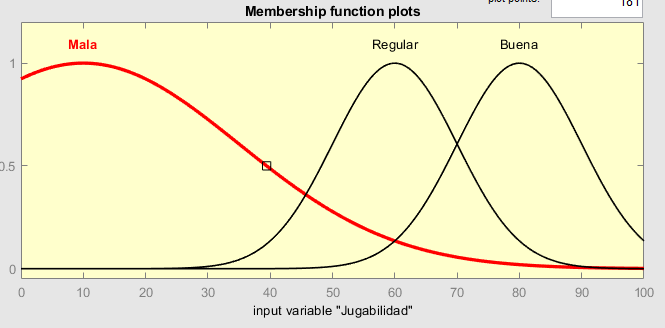
\includegraphics[width=0.8\textwidth]{IMG/P11.png}
	\end{figure}
	
	\newpage
	
	\item Comida: Malo ($\mu = 15$, $\sigma = 15$), Normal ($\mu = 45.5$, $\sigma = 15$), Buena ($\mu = 66$, $\sigma = 10$) y Excelente ($\mu = 90$, $\sigma = 15$).
	\begin{figure}[h]
		\centering
		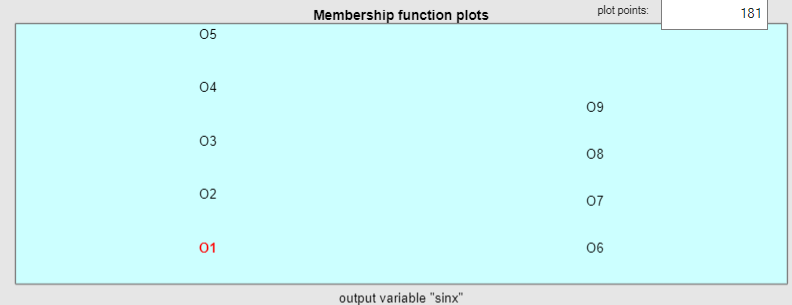
\includegraphics[width=0.8\textwidth]{IMG/P12.png}
	\end{figure}
	
	\item Propina: Baja ($\mu = 5$, $\sigma = 2$), Normal ($\mu = 10$, $\sigma = 2$) y Alta ($\mu = 16$, $\sigma = 1.5$).
	\begin{figure}[h]
		\centering
		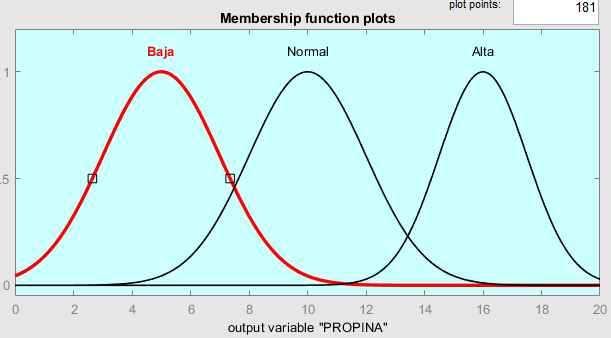
\includegraphics[width=0.8\textwidth]{IMG/P13.png}
	\end{figure}
\end{enumerate}

Las funciones de membresía de SERVICIO y COMIDA fueron modeladas con Gaussianas al igual que las funciones de membresía para la PROPINA.

Se mantuvo el método de desfuzzificación del centroide (centro de masa) para todas las funciones con la inferencia de Mandani para los resultados obtenidos mediante el fuzzy toolbox de matlab.\\

\newpage

\subsection{Reglas de inferencia.}

A continuación se muestran las doce reglas que se construyeron para este problema:

\begin{enumerate}
	\item R1: Si \textbf{SERVICIO} es \textbf{\textit{MALO}} y la \textbf{COMIDA} es \textbf{\textit{MALA}}, la \textbf{PROPINA} es \textbf{\textit{BAJA}}.
	\item R2: Si \textbf{SERVICIO} es \textbf{\textit{BUENO}} y la \textbf{COMIDA} es \textbf{\textit{NORMAL}}, la \textbf{PROPINA} es \textbf{\textit{NORMAL}}.
	\item R3: Si \textbf{SERVICIO} es \textbf{\textit{REGULAR}} y la \textbf{COMIDA} es \textbf{\textit{NORMAL}}, la \textbf{PROPINA} es \textbf{\textit{NORMAL}}.
	\item R4: Si \textbf{SERVICIO} es \textbf{\textit{REGULAR}} y la \textbf{COMIDA} es \textbf{\textit{BUENA}}, la \textbf{PROPINA} es \textbf{\textit{NORMAL}}.
	\item R5: Si \textbf{SERVICIO} es \textbf{\textit{BUENO}} y la \textbf{COMIDA} es \textbf{\textit{EXCELENTE}}, la \textbf{PROPINA} es \textbf{\textit{ALTA}}.
	\item R6: Si \textbf{SERVICIO} es \textbf{\textit{MALO}} y la \textbf{COMIDA} es \textbf{\textit{EXCELENTE}}, la \textbf{PROPINA} es \textbf{\textit{BAJA}}.
	\item R7: Si \textbf{SERVICIO} es \textbf{\textit{BUENO}} y la \textbf{COMIDA} es \textbf{\textit{MALA}}, la \textbf{PROPINA} es \textbf{\textit{BAJA}}.
	\item R8: Si \textbf{SERVICIO} es \textbf{\textit{MALO}} y la \textbf{COMIDA} es \textbf{\textit{NORMAL}}, la \textbf{PROPINA} es \textbf{\textit{BAJA}}.
	\item R9: Si \textbf{SERVICIO} es \textbf{\textit{MALO}} y la \textbf{COMIDA} es \textbf{\textit{BUENA}}, la \textbf{PROPINA} es \textbf{\textit{BAJA}}.
	\item R10: Si \textbf{SERVICIO} es \textbf{\textit{BUENO}} y la \textbf{COMIDA} es \textbf{\textit{BUENA}}, la \textbf{PROPINA} es \textbf{\textit{ALTA}}.
	\item R11: Si \textbf{SERVICIO} es \textbf{\textit{REGULAR}} y la \textbf{COMIDA} es \textbf{\textit{MALA}}, la \textbf{PROPINA} es \textbf{\textit{BAJA}}.
	\item R12: Si \textbf{SERVICIO} es \textbf{\textit{REGULAR}} y la \textbf{COMIDA} es \textbf{\textit{EXCELENTE}}, la \textbf{PROPINA} es \textbf{\textit{ALTA}}.
\end{enumerate}

\newpage

\subsection{Gráficos del problema del mesero}

La gráfica de superficie resultante del problema con entradas y salidas Gaussianas y la base de reglas ya mencionada toma la siguiente forma:

\begin{figure}[h]
	\centering
	\begin{subfigure}{0.42\textwidth} % Reducido de 0.45
		\centering
		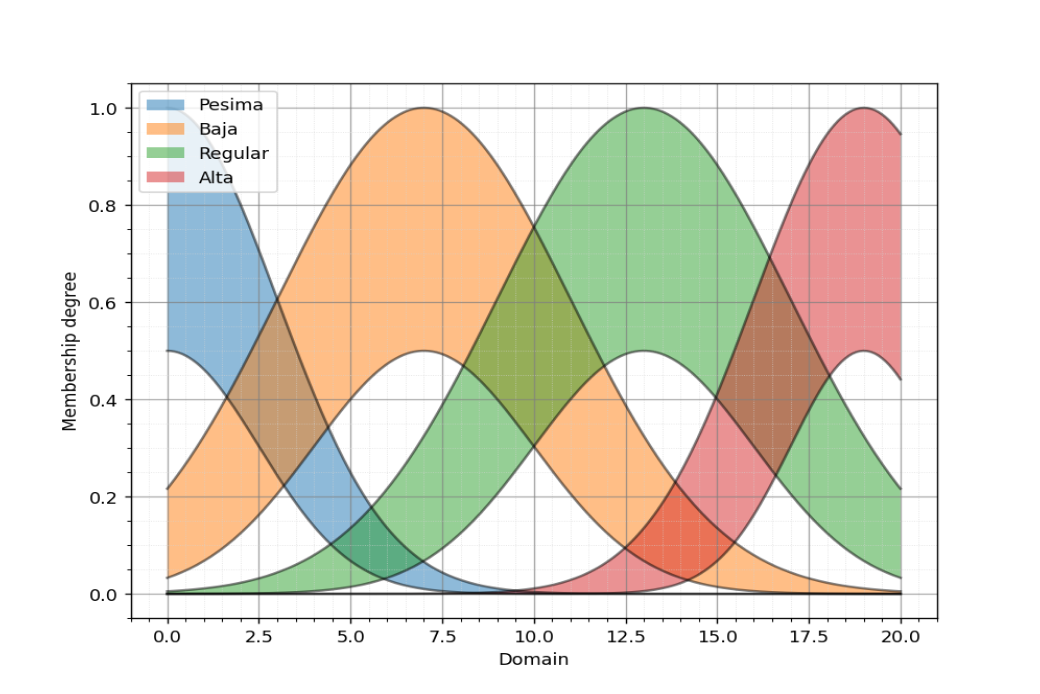
\includegraphics[width=1.3\textwidth]{IMG/P14.png}
		\label{fig:G1}
	\end{subfigure}
	\hfill
	\begin{subfigure}{0.42\textwidth} % Reducido de 0.45
		\centering
		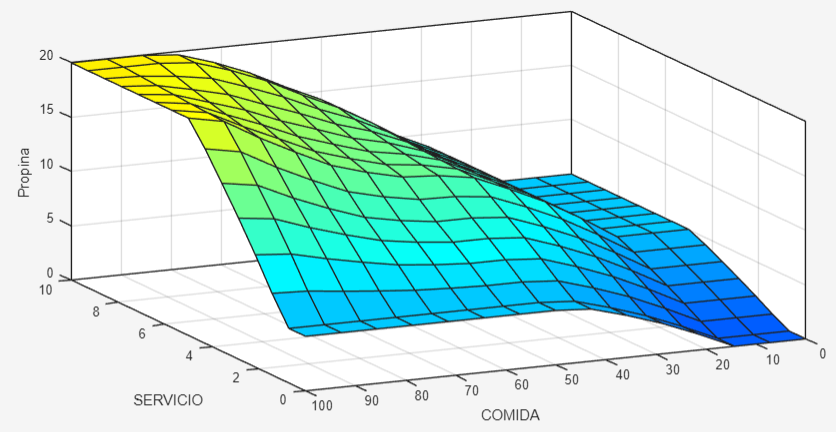
\includegraphics[width=1.2\textwidth]{IMG/P15.png}
		\label{fig:G2}
	\end{subfigure}
	\label{fig:comparacion1}
\end{figure}

La gráfica producida por el sistema difuso resulta suave en su mayoría, no difiere mucho de la encontrada en la tarea 2. 

\newpage

\subsection{Implementación del problema del mesero con desfuzzificación del centro de sumas paso a paso}

Como se menciono en un inicio, el principal objetivo de esta actividad es implementar uno mismo el sistema de lógica difusa para comparar los resultados con respecto de los mostrados por el fuzzy toolbox de matlab.\\

El primer paso  identificar las variables de discurso SERVICIO, COMIDA y PROPINA para inicializarlas en 0.\\

Con referencia a lo explicado en el libro de \cite{Cisneros2004}, se implemento la función de membresía Gaussiana tal y como la define a continuación:

\[
f(x, \mu, \sigma) = e^{\left( \frac{(x - \mu)^2}{2\sigma^2} \right)}
\]

Posteriormente, se definieron los rangos de cada una de las funciones de membresía, dado que solo se usan funciones gaussianas, se dejaron los rangos tal cual se había presentado anteriormente:

\begin{enumerate}
	\item Servicio: Malo ($\mu = 1.5$, $\sigma = 2$), Regular ($\mu = 5$, $\sigma = 1.5$) y Bueno ($\mu = 7.5$, $\sigma = 1.5$).
	\item Comida: Malo ($\mu = 15$, $\sigma = 15$), Normal ($\mu = 45.5$, $\sigma = 15$), Buena ($\mu = 66$, $\sigma = 10$) y Excelente ($\mu = 90$, $\sigma = 15$).	
	\item Propina: Baja ($\mu = 5$, $\sigma = 2$), Normal ($\mu = 10$, $\sigma = 2$) y Alta ($\mu = 16$, $\sigma = 1.5$).

\end{enumerate} 


Siguiendo con el proceso, fueron implementadas cada una las 12 reglas que ya se mostraron previamente, haciendo uso de la operación de conjuntos difusos $AND$, para esto, la activación de las reglas del sistema se determinan de la siguiente forma:

\[
\text{Activación de regla}  = \min( \mu_A(X), \mu_B(Y) )
\]

\newpage

Posteriormente, se implemento el método de desfuzzificación del centroide o centro de área como sigue.

Siguiendo la definición descrita en \cite{Cisneros2004}, el centro de área llega a una conclusión "verdadera" para el razonamiento difuso para el valor $\bar{u}$ que se encuentra dentro del rango que es promedio de todos los valores. Dicho promedio se construye mediante cada valor $u$ que es ponderado por el área que se encuentra por encima de el como se muestra a continuación:


$$\bar{u} = \frac{\int_{u_1}^{u_n}u\mu_{U}(u)du}{\int_{u_1}^{u_n}\mu_{U}(u)du}$$

De forma que el denominador en la expresión representa el área por debajo de la gráfica que se produce.\\

Debido a que en el presente trabajo se utilizaron unicamente funciones gaussianas, se recurre a realizar la integración sobre un dominio numérico de valores continuos que van de 0 a 20 mediante una aproximación a la integral mediante sumas discretas:

$$Crisp \approx \frac{\sum_{i=1}^{n} x_i \cdot \mu(x_i)}{\sum_{i=1}^{n} \mu(x_i)}$$

donde:

\begin{itemize}
	\item \( x_i \) son los valores discretos de la variable de salida generados en el intervalo.
	\item \( \mu(x_i) \) es el valor de la función de membresía en \( x_i \).
	\item \( n \) es el número total de puntos utilizados en la discretización.
\end{itemize}


Una vez que el sistema esta listo y programado, se procede a hacer la comparativa con el toolbox de matlab.

\newpage

\subsection{Comparativa para el problema del mesero}


A continuación se presentan los resultados que da el sistema programado paso a paso en matlab contra el resultado para el mismo sistema por parte del fuzzy toolbox en 3 escenarios distintos.

\subsubsection{Caso mínimo}

Para el caso mínimo, se propone un $SERVICIO = 0$ y una $COMIDA = 0$ para ver como se comportan ambas versiones ante la situación extrema de puntuar todo con 0.

\begin{figure}[h]
	\centering
	\begin{subfigure}{0.40\textwidth} % Reducido de 0.45
		\centering
		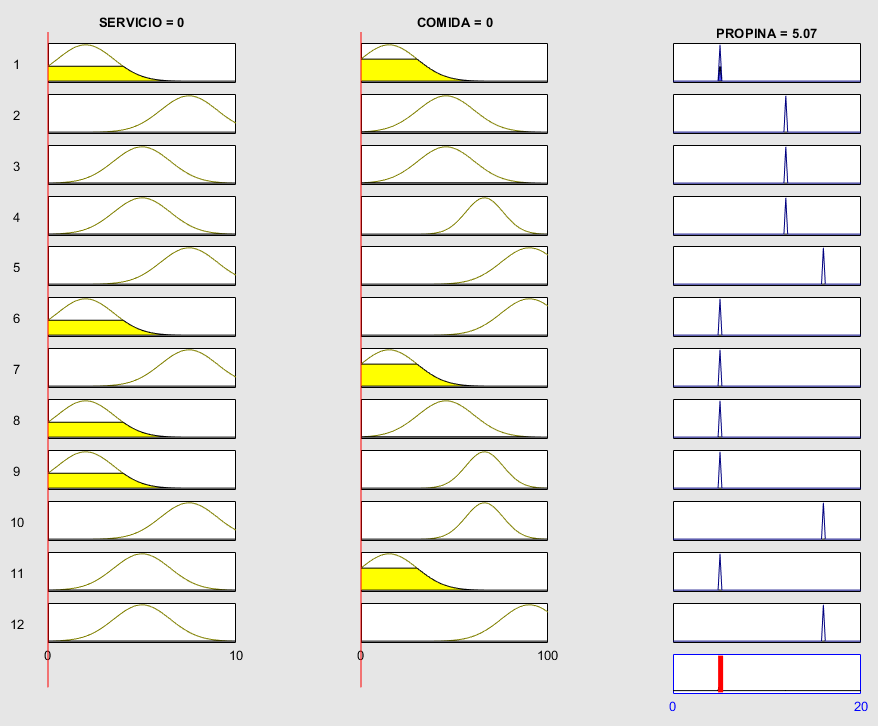
\includegraphics[width=1.4\textwidth]{IMG/RP11.png}
		\label{fig:G3}
	\end{subfigure}
	\hfill
	\begin{subfigure}{0.42\textwidth} % Reducido de 0.45
		\centering
		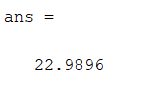
\includegraphics[width=0.8\textwidth]{IMG/M11.png}
		\label{fig:G4}
	\end{subfigure}
	\label{fig:comparacion2}
\end{figure}

A la izquierda se muestran los resultados del toolbox y a la derecha el resultado del sistema programado paso a paso. 
Fuzzy toolbox reporta un valor de 5.09 para el caso planteado, mientras que el sistema programado paso a paso muestra un valor de 5.0419. La diferencia entre ambos casos es mínima (menos de una décima), por lo que se puede afirmar que llegan al mismo resultado. Un servicio de 0 y una comida de 0 llegan a dar como resultado una propina de 5.065\% en promedio (baja).

\newpage

\subsubsection{Caso medio}
Para el caso mínimo, se propone un $SERVICIO = 4$ y una $COMIDA = 52$ para ver como se comportan ambas versiones ante situación media.

\begin{figure}[h]
	\centering
	\begin{subfigure}{0.40\textwidth} % Reducido de 0.45
		\centering
		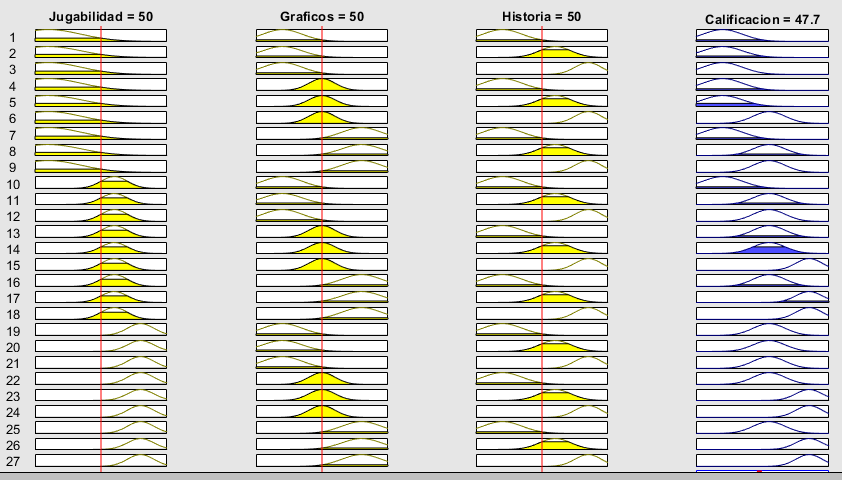
\includegraphics[width=1.4\textwidth]{IMG/RP12.png}
		\label{fig:G5}
	\end{subfigure}
	\hfill
	\begin{subfigure}{0.42\textwidth} % Reducido de 0.45
		\centering
		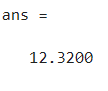
\includegraphics[width=0.8\textwidth]{IMG/M12.png}
		\label{fig:G6}
	\end{subfigure}
	\label{fig:comparacion3}
\end{figure}

A la izquierda se muestran los resultados del toolbox y a la derecha el resultado del sistema programado paso a paso. El toolbox reporta un valor de 8.4 para el caso planteado, mientras que el sistema programado paso a paso muestra un valor de 8.5422. La diferencia entre ambos casos es mínima (menos de dos décimas), por lo que se puede afirmar que llegan al mismo resultado. Un servicio de 4 y una comida de 52 llegan a dar como resultado una propina de 8.47\% en promedio (media).

\newpage

\subsubsection{Caso máximo}
Para el caso mínimo, se propone un $SERVICIO = 10$ y una $COMIDA = 100$ para ver como se comportan ambas versiones ante situaciones tan extremas.

\begin{figure}[h]
	\centering
	\begin{subfigure}{0.40\textwidth} % Reducido de 0.45
		\centering
		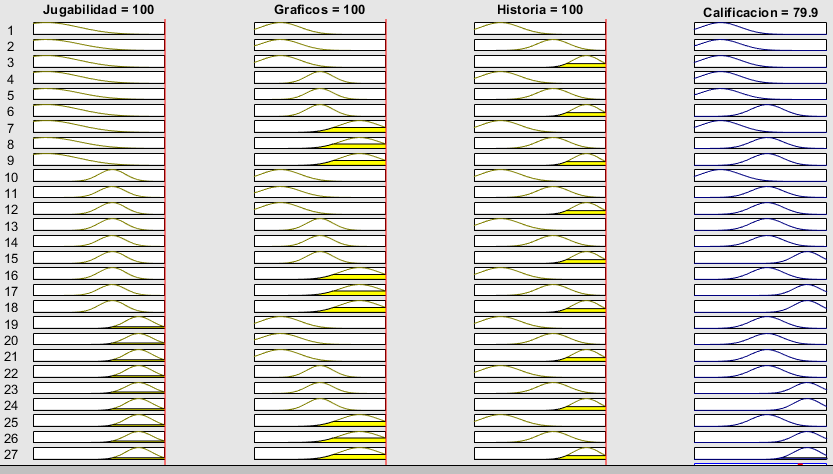
\includegraphics[width=1.4\textwidth]{IMG/RP13.png}
		\label{fig:G7}
	\end{subfigure}
	\hfill
	\begin{subfigure}{0.42\textwidth} % Reducido de 0.45
		\centering
		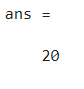
\includegraphics[width=0.8\textwidth]{IMG/M13.png}
		\label{fig:G8}
	\end{subfigure}
	\label{fig:comparacion4}
\end{figure}

A la izquierda se muestran los resultados del toolbox y a la derecha el resultado del sistema programado paso a paso. El toolbox reporta un valor de 15.8 para el caso planteado, mientras que el sistema programado paso a paso muestra un valor de 15.90. La diferencia entre ambos casos es mínima, por lo que se puede afirmar que llegan al mismo resultado. Un servicio de 10 y una comida de 100 llegan a dar como resultado una propina del 15.95 \% (Alta) en promedio.


\newpage

\section{Conclusiones}

La implementación del método de desfuzzificación fue un reto interesante, puesto que a nivel conceptual se puede entender como si fuera una suma ponderada de las funciones de membresía entre sus sumas no ponderadas para llegar finalmente a el valor de la propina que se va a dejar en forma interpretable.

Los resultados encontrados por ambos métodos (fuzzy toolbox y el propio) con los mismos parámetros en los 3 casos planteados llegan prácticamente al mismo resultado con una diferencia de menos de una unidad, por lo que la lógica implementada paso a paso parece ser que esta bien estructurada al tomar como punto de referencia los resultado del toolbox.

Un reto no abordado pero pendiente por implementar, es considerar el caso donde las funciones no son gaussianas, si no que son trapezoidales o triangulares para poder acoplar adecuadamente la lógica de la desfuzzificación más adelante.





\newpage

\section{Referencias}

\bibliographystyle{apalike}  % Estilo de cita, puedes cambiarlo si lo prefieres.
\bibliography{Biblio}         % Aquí incluyes el archivo .bib (sin extensión).

\newpage

\section{Anexos}

Este reporte se envía con los códigos anexos que corresponden a:

\begin{enumerate}
	\item Archivo .fiz del sistema difuso para el problema 1 con la desfuzificación 
	\item Código en matlab para ejecutar el sistema difuso programado para el problema 1

\end{enumerate}



\end{document}

